% Copied version from 2018-10-28 based on
%   7ed696cbe8d60fd5a5c9d28db5263d17c0caa490
% of the GUPBH paper repo

\providecommand{\Mbh}{M_{\rm BH}}
\providecommand{\Mpl}{m_\mathrm{Pl}}
\providecommand{\ellp}{\ell_\mathrm{Pl}}
\providecommand{\Mf}{M_d}
\providecommand{\sgn}{\mathrm{sgn}}
\providecommand{\diff}{\mathrm{d}}
\providecommand{\tpi}{(2\pi)}
\providecommand{\dovertwo}{\frac{d}{2}}
\providecommand{\Sin}{%
	\mathop{\sbox0{$\cos$}\makebox[\wd0][r]{$\sin$}}%
}

% Chapter start
This chapter summarizes efforts in modeling black hole solutions in a
first order quantum gravity theory. This phenomenological model is 
obtained by adding momentum-dependent terms to Heisenbergs uncertainty
principle, resulting in a certain $f(R)$ gravity modification which is
subsequently studied in its geometric and thermodynamics properties.
%\footnote{
%	Despite probably being obvious, it should be mentioned
%	 at the very beginning that this chapter does not
%	consecutively build up on the research infrastructure presented in the 
%	previous chapters (and which evventually lead to 
%	chapter~\ref{chapter:bnslt}).
%	This work was carried out primarily analytically in a ``paper and pen
%	physics'' fashion.
%}
For an interoduction into the problem and a review of previous work, see
Section~\vref{sec:gr-intro-intro}.
As a motivation, this chapter starts with higher dimensional spacetime.
This chapter is based on parts of \cite{Koppel:2017rsf} as well as the upcoming
publication \cite{Knipfer2019}.

\section{Motivation: Higher dimensional Black Hole 
spacetimes}\label{sec:motivation-qbh}
Higher dimensional black hole solutions play an important role in theoretical 
research for an array of reasons. On the more formal side, they are a key 
element of proposals aiming to a unified description of fundamental 
interactions, \textit{e.g.}, Superstring theory and related paradigms, like the 
gauge/gravity duality.
On the more phenomenological side, microscopic higher dimensional black holes 
would be the ``smoking  gun'' for the terascale quantum gravity 
\cite{BaF99,DiL01,GiT02}  and a viable resolution of the hierarchy problem 
\cite{AAD98,ADD98,ADD99,RaS99a,RaS99b,ACD01}.

\begin{marginfigure}
	\includegraphics[width=\linewidth]{figures-from-master-thesis/cavaglia-evaporation.pdf}
	\caption[
	Brane world physics, figure modified from \cite{cavaglia}
	\cite{Koeppel2014})
	]{Cartoon of the 4-dimensional spacetime (brane), where standard model (SM)
		particles are allowed to propagate on, while gravitational degrees of
		freedom (\ie gravitons, g) can propagate in the extra dimensions. The 
		ball shall indicate the extension of the hyper-spherical black hole.
		Modified from \cite{cavaglia}.}\label{fig:brane-world}
	%
	%
	\vspace{1cm}
	\includegraphics[width=\linewidth]{figures-from-master-thesis/hossi-minibh.pdf}
	\caption[
	Embedding of mini black holes in compactified extra dimensions, figure
	modified from \cite{Hos04}.
	]{Embedding of a black hole with $r_H \ll R_c$, where $R_c$ is the compactification
		radius of an extra dimension. In such a case, the black hole does not notice
		the extra dimensional periodic boundary geometry. Colorized from
		\cite{Hos04}.
	}\label{fig:minibh}
\end{marginfigure}

The common ideas of higher dimensional gravity can be motivated by a number of
concepts. For instance, gravitational radiation can penetrate the $n$-dimensional
bulk space, while standard model forces are restricted to the 3-dimensional bulk
(Figure \ref{fig:brane-world}). On the other hand, micro black holes are supposed
to be so small that the geometry of the extra dimensions plays no role.
This concept is depicted with a toroidial extra dimension in Figure \ref{fig:minibh},
where the black hole event horizon $r_H$ is much smaller then the compact torus radius
$R_C$. For reviews about microscopic black holes in particle physics, see
\cite{Lan02,Cav03,Kan04,Hos04,CaS06,Win07,BlN10,Cal10a,Par12,NMS13,BlN14,KaW15}.

In this work, we consider hyper-spherical black hole spacetimes, that is,
Schwarz\-schild-Tangherlini spacetimes~\cite{Tangherlini:1963bw, Emparan:2008eg}
\begin{equation}\label{eq:STM-f}
\diff s^2 = -\left( 1 - f(r) \right)\diff t^2 + 
(1 - f(r))^{-1}\diff r^2 + r^2 \diff\Omega^2_{n-1}\,,
\end{equation}
with the $(n-1)$-dimensional hyper-spherical surface element $\diff\Omega^2_{n-1}$
and a gravitational function, which is $f(r)=2 G_\mathrm{N} M/r$ in the classical
case.
These theories can fit in both the large extradimension scenario, \ie the
1998 pioneered ADD model (Arkani-Hamed, Dimopoulos, Dvali \cite{ADD98,ADD99,AAD98}),
and in the universal extradimension scenario \cite{ACD01}, \ie an extension to
the 1921 developed Kaluza Klein theory \cite{Overduin:1998pn,historyGoenner}
which proposes only one space-like extradimenion.

For sake of simplicity, however, we assume as a new fundamental scale $M_* = 
M_\text{Pl}^{2/(n+2)} C_n V_n$ according to the large extradimension model 
only, where $M_\text{Pl}$ is  the $4$-dimensional Planck mass scale and $V_n$ 
is the volume of the $n$ extra dimensions.  For a torodial compactification
(Figure \ref{fig:minibh}) with an 
extend $R_\text{c}$, the volume is $V_n = (2\pi R_c)^n$ and 
$C_n=\mathcal{O}(1)$ a dimensionless prefactor.
Unless differently specified, all quantities 
are expressed in units of the fundamental Planck mass $M_*$, or of the 
fundamental length $L_*=1/M_*$. According to this notation, the effective 
gravitational coupling constant reads $G_*=1/M_*^2$.

%One of the biggest quests of our current age is to unite General Relativity 
%and Quantum Field Theory.
%Both theories agree extraordinary well with experimental data at their 
%respective scales.
%Black Holes are where both scales meet. The standard GR Schwarzschild black 
%hole has two problems:
%1) a singularity at its center which tells us that GR breaks down there and 
%2) the (semiclassical) Hawking temperature $T_\text{H}\sim 1/M$ diverges as 
%the black hole evaporates. 
%Quantum Gravity effects might cure both of these problems.

%One particular model we are looking at is the Generalized Uncertainty 
%Principle (GUP)
%$\delta x \delta p \geq 1+\beta (\delta p)^2$. In 3+1 dimensions this model 
%changes the horizon structure
%as has been shown in (ref here).

%We will review the model, show that it does not work in higher dimensions and 
%propose a modification to
%higher dimensions.

%\todo{Remove this summary but keep the names of the proposals}
%The paper is organized as follows. In Section \ref{sec:GUPhigher} we summarize 
%the existing proposals for a GUP in higher dimensional spacetimes. In Section 
%\ref{sec:GUP}, we consider the general set up to deform Einstein's equation in 
%the presence of nonlocal effects and we implement the GUP proposed by the 
%\emph{Kempf-Mann-Mangano proposal} \cite{KMM95}. In Section ... we consider the 
%proposal of Scardigli and Casadio \cite{ScC03}, and Carr and Lake 
%\cite{Car13,Car14,LaC15,LaC16}  and in Section that of 
%Maziashvili \cite{Maz12,DMS15,Maz15}. Finally in Section .. , we draw our 
%conclusions.

\section{A brief introduction into the Generalized Uncertainty principle}
%
\begin{marginfigure}[3cm]
	% trim={<left> <lower> <right> <upper>}
	\includegraphics[width=\textwidth,trim={0 1cm 0 
	0},clip]{figures-from-holographyPaper/completeness-schwarzschild.pdf}
	\includegraphics[width=\textwidth]{figures-from-holographyPaper/completeness-repaired.pdf}
	\caption[
	Size vs Energy relations at the Planck scale, \publishedIn{FKN16}
	]{
		Size vs. Energy relation in Planck units. Upper panel: Particle size (Compton
		wavelength $\lambda_C \sim M^{-1}$) in red, vs. black hole size (Schwarzschild
		radius $r \sim M$). The shaded area is inaccessible in the particle
		acceleration/compression process. At the sub-Planckian ($M<1 M_P$) regime, a
		length scale ambiguity arises.
		The lower panel shows the solution proposed by the self-complete gravity paradigm. 
		(Figure published in \cite{FKN16}).
	}\label{fig:completeness-intro}
\end{marginfigure}%
%
Mathematically, the Generalized Uncertainty Principle (motivated in Section
\ref{sec:gr-intro-intro}) can be casted as commutator relation
\begin{equation}
[x^i, p_j] = i\, \hbar\, \delta^i_{\, j} \, (1+f( \vec{p}^2))
\label{eq:commrel}
\end{equation}
where the function $f$ is customarily assumed as $f(\vec{ p}^{\,\,2})\simeq 
\beta \vec{ p}^{\,\,2}+\dots$ at first order. From \eqref{eq:commrel}, one 
obtains that spatial resolution better than $\sqrt{\beta}$ is no longer 
possible, since the uncertainty relations reads 
\begin{equation}
\Delta x \Delta p \geq \frac \hbar2 (1+\beta(\Delta p)^2).
\label{eq:gup}
\end{equation}
In order to study nonlocal gravity, one can formally shift the nonlocalities
from the energy momentum tensor to the Einstein tensor, \ie consider a
nonlocal version of Einsteins equations \cite{Kra87,Tom97,Bar03,Mod12a}
\begin{equation}
G_\mathrm{N}^{-1}\left(L^2\Box\right)G_{\mu\nu}=8\pi T_{\mu\nu}
\label{eq:nleinstein}
\end{equation}
where the Newton's constant becomes a differential operator, $\Box$ is the 
covariant d'Alembertian and $L$ is a length scale. Eq. \eqref{eq:nleinstein} 
can be either used to described large scale degravitating effects 
\cite{ADD02,DHK07,Bar05,Bar12} or short scale modified gravity theories 
\cite{GHS10,MMN11,Nic12,CMN14,FKN16}. One can select a specific 
profile of $G_\mathrm{N}^{-1}\left(L^2\Box\right)$ to reproduce the GUP 
momentum space deformation
\begin{equation}
\diff^3 \vec{p} \to \frac{\diff^3 \vec{p}}{1+\beta p^2}\ 
\label{eq:kempf}
\end{equation}
for the static potential due to virtual particle exchange by setting 
$L=\sqrt{\beta}$. The resulting non-rotating black hole metric
(reviewed in the next Section) allows for 
horizon extremisation with consequent formation of a zero temperature black 
hole remnant at the end of the evaporation \cite{IMN13}. Such a black hole 
solution not only supersedes the aforementioned limitations of the scenario 
proposed in \cite{AdS99,APS01}, but offers additional interesting properties: 
it removes the scale ambiguity of the Schwarzschild metric and fulfills the 
\emph{gravity ultraviolet self completeness} by preventing black hole radii smaller 
than the Planck length (Figure \ref{fig:completeness-intro});
it allows for a semiclassical description of the whole 
evaporation process for the presence of the SCRAM phase\footnote{The black hole 
	SCRAM is a cooling down phase during the final stages of the evaporation. The 
	term SCRAM has been introduced in \cite{Nic09} by borrowing it from nuclear 
	reactor technology. SCRAM is a backronym for ``Safety control rod axe man'', 
	introduced by Enrico Fermi in 1942 during the Manhattan Project at Chicago 
	Pile-1. It still indicates an emergency shutdown of a nuclear reactor.} before 
the remnant formation. If the theory of study has a free parameter, it can be
tuned in a way that the minimal length black hole mass $M_0$ coincides with the
fundamental mass of general relativity $M_*$ (self completeness). For certain
theories, also the size of the minimal length black hole $r_0$ can be identified
as the fundamental length scale $L_*$ \cite{FKN16}.

%Given the above background, it is natural to consider the case of GUP effects 
%in higher dimensional black hole metrics. To this purpose it has to be noted 
%that there is no unique prescription for the GUP in the presence of 
%extra-dimensions \cite{Koppel:2017rsf}. As a result, before entering presenting 
%corrections to higher dimensional black holes, we will provide an analysis of 
%the existing proposals for the GUP in $d$-dimensions with $d=4+n$ 
%\cite{ScC03,Maz13,Car13,Car14,LaC15,LaC16,Maz12,DMS15,Maz15}.


\section[
  Review of GUP Black Holes in the KMM measure
]{Review of GUP Black Holes in the Kempf-Mangano-Mann momentum measure}
\label{sec:GUP}

To begin with, we review the calculation of the GUP modified Schwarzschild 
solution~\cite{IMN13} in $(3+1)$ dimensions.
We chose a specific profile of the operator $\mathbb{G}^{-1}(L^2\Box)$
such that effectively the momentum measure is modified as in the 
model by Kempf Mangano Mann (KMM)~\cite{KMM95}. 

\subsection{3+1 Dimensional GUP inspired Black Holes}
\begin{figure*}[t]
	% Unfortunately the refs to the labels defined here dont work properly
	% There is the subcaption package which seems to superseed the subfigure
	% environment but breaks tuftes figure*.
	\begin{subfigure}{.5\textwidth}
		% This new figure of Sven replaces Marcos gup-figures/g00kempf.pdf
		\caption{Kempf-Mangano-Mann metric\label{fig:g00kempf}}
		\vspace*{-2mm}
		\includegraphics[width=\linewidth]{svens-new-mma-figures/g00-GUP-n0.pdf}
	\end{subfigure}
	\begin{subfigure}{.5\textwidth}
		\caption{Temperature of the KMM black hole\label{fig:kempftemp}}
		\vspace*{-2mm}
		\includegraphics[width=\linewidth]{svens-new-mma-figures/Temp-n0.pdf}
	\end{subfigure}
	\caption[
	  Two panels: KMM metric and temperature (done myself),
	  \publishedIn{Knipfer2019}
	]{
		(a) The Kempf GUP metric~\protect\eqref{eq:gupschwarzschild} component 
		$g_{00}(r)$ shown for different black hole masses. For comparison,
		the dashed line show the corresponding curves for the unmodified
		Schwarzschild metric, \ie $\mathcal M(r)=1$ in
		Eq.~\protect\eqref{eq:gupschwarzschild}. For heavy masses, there are
		two horizons (blue line, locations marked at $g_{00}=0$), for a
		critical mass these horizons merge to a single one (red line). For
		a subcritical mass, there is no horizon (red line). Since there is
		still a divergent Ricci scalar, this is a naked singularity.
		
		(b) Temperature of the GUP black hole in $n=3$ spatial dimensions as a
		function of the outer horizon radius $r_+$.
		For comparison, the Hawking temperature of
		a traditional Schwarzschild black hole displayed.
		The blue and red dots mark the cold and hot remnant,
		respectively.
	}\label{fig:kempf-general}
\end{figure*}
%
Equation~\eqref{eq:nleinstein} can be cast in the form
\begin{equation}\label{eq:nlee}
R_{\mu\nu} - \frac{1}{2} g_{\mu\nu} R = 8 \pi \mathbb{G}(L^2\Box) T_{\mu\nu}~,
\end{equation}
that is equivalent to coupling Einstein gravity to a non-standard energy
momentum tensor. In case of a static, spherically symmetric spacetime, one has
\begin{equation}
\label{eq:cltoo}
T^{\ 0}_0=-M \delta^{(3)}(\vec{x}) ~, %=-\frac{M}{4 \pi r^2} \delta (r)~,
\end{equation}
corresponding to a vanishing mass distribution, apart from the origin where
a curvature singularity is present \cite{BaN93,BaN94,DeB08}. The action of
the operator $\mathbb{G}(L^2\Box)$ determines a smearing of the source
term that reads
\begin{equation}
\mathbb{T}^{\ 0}_0(\vec{x})\equiv\frac{1}{G_\mathrm{N}} \ \mathbb{G}(L^2\Box) T^{\ 0}_0  = -\rho(\vec{x}) \,.
\end{equation}
Since the Dirac delta distribution $\delta^{(3)}(\vec{x})$ can be represented
as the Fourier tranform of the plane wave,
\begin{equation}
    \delta^{(3)}(\vec{x}) = \frac{1}{(2\pi)^{3}}\int \diff^3\vec{p}\ e^{i 
    \vec{x}\cdot\vec{p}} \,.
    \label{eq:delta}
\end{equation}
one can apply the Kempf momentum space measure \eqref{eq:kempf} in order
to ``smear out'' the matter distribution,
\begin{equation}
    \rho_\beta(\vec{x}) = \frac{M}{(2\pi)^{3}}\int 
    \frac{\diff^3\vec{p}}{1+\beta p^2}  e^{i \vec{x}\cdot\vec{p}}=
    M \frac{e^{-\frac{x}{\sqrt{\beta}}}}{4\pi x \beta} \,,
    \label{eq:smeared}
\end{equation}
with an energy scale $\beta^{-1/2}$ (or length scale $\sqrt{\beta}$,
respectively). The nonlocal operator
\begin{equation}
\label{eq:goperator}
\mathbb{G}(L^2\Box) = \frac{G_\mathrm{N}}{1 - L^2 \Box}
\end{equation}
is chosen to mimic GUP effects (the modified momentum measure) and is
equivalent to the usual Einstein's equations  with $\rho_\beta$ as source.

From \eqref{eq:goperator} it can be seen that in the low energy regime
$-\Box\ll L^{-2}$, \eqref{eq:nlee} match Einstein equations and
$\mathbb{G}(L^2\Box) \to G_\mathrm{N}$. Conversely for $-\Box\sim L^{-2}$,
strong non-local corrections enter the game, gravity becomes increasingly
weaker ($\mathbb{G}(L^2\Box) \ll G_\mathrm{N}$), and the source can no
longer be compressed as in \eqref{eq:cltoo}. We note that the profile
in \eqref{eq:goperator} modifies the momentum measure in the same way
as in \eqref{eq:kempf}, namely the KMM model \cite{KMM95}.

Solving Einstein's Field Equations with this source \textit{\`a la} 
Schwarzschild  gives the four dimensional line element
\begin{align}
    \diff s^2 &= -\left( 1-\frac{2G_\mathrm{N}\mathcal{M}(r)}{r}\right)\diff t^2 
    + \left( 1-\frac{2G_\mathrm{N}\mathcal{M}(r)}{r}\right)^{-1}\diff r^2 + r^2 \diff \Omega^2\ ,\quad
    \label{eq:gupschwarzschild}
\end{align}
\ie the generic static, spherically symmetric metric with
\begin{align}
    \mathcal{M}(r) &= \int_{B_r}\diff^3\vec{x}\,\rho(\vec{x}) 
\end{align}
representing the cumulative mass distribution, \ie the matter contained
within a 3-ball $B_r$ of radius $r$. 
%
Given \eqref{eq:gupschwarzschild}, the conservation of the energy momentum
tensor implies its form, namely $\mathbb{T}_\mu^\nu=\mathrm{diag} \left(-\rho, p_r, p_\perp, p_\perp\right)$
with radial pressure $p_r=-\rho$ and perpendicular pressure
$p_\perp=-\rho-\frac{1}{2}r (\diff \rho/\diff r)$.
%
By assuming $\rho(\vec{x})$ given in \eqref{eq:smeared}, one finds
\footnote{
	Here, $\gamma(s;x)$ is the lower incomplete gamma function,
    see Appendix \ref{apx:symbols} for general definitions.
}
\begin{align}
    \mathcal{M}(r)% &= \int_{B_r}\diff^3\vec{x}\,\rho_\beta(\vec{x})
    %\\ &= 
    &= M\gamma\left(2;\frac{r}{\sqrt{\beta}}\right)\ 
    = M\left[ 1 - 
    e^{-\frac{r}{\sqrt{\beta}}} - \frac{r}{\sqrt{\beta}}
    e^{-\frac{r}{\sqrt{\beta}}}\right]\,.
    \label{eq:mass}
\end{align}
%n}
The behaviour of the metric (in comparison to the same mass Schwarzschild
metric) can best be seen when plotting the
metric coefficient $g_{00}(r)$ as in Figure~\ref{fig:kempf-general}.
The horizon structure resembles that of the (mass dominated)
Reissner-Norstr\"{o}m solution:
there exist an outer event horizon $r_+$ and an inner Cauchy horizon $r_-$. 
The two eventually merge at the critical mass parameter
$M=M_0= 1.68 \sqrt{\beta}/G_\mathrm{N}$, corresponding to an extremal
configuration. The curvature still diverges at the origin
(Ricci scalar $R\to 1/4\pi \beta r$), but less ``brutally'' than
in the Schwarzschild case. 
This can be seen from the fact that, in contrast to the Schwarzschild
case, the metric is no longer divergent at the origin. That is, only the
first and higher derivatives of the metric are singular at this point,
which implies a ``softer'' singularity. \footnote{
  Another quantitative argument is the Kretschmann scalar, which diverges
  for Schwarzschild as $K\sim 1/r^6$ and for the GUP only as
  $K \sim 1/r^2$.	
}

Such a property of the GUP inspired black holes is similar to that of the
recently proposed holographic metric~\cite{NiS12,FKN16}.
For other quantum corrected black hole solutions, however, the metric and
all its derivatives are regular at the origin implying a removal of the
curvature singularities~\cite{NSS06b,Nic09,NiS10,Nic12,NSW19}.
Despite the singular behavior of the spacetime \eqref{eq:gupschwarzschild}
the gravitational field, $\vec{g}=\vec{\nabla} g_{00}$, can be computed in
a neighborhood of the origin: it turns out to be constant and repulsive.
Much in the same way as the aforemetioned regular geometries, the
quantum fluctuations of the manifold provide an outer pressure that
prevents the energy density to collapse in a Dirac delta profile.

The existence of an extremal configuration has an impact on the
thermodynamics.
The Hawking temperature does not diverge as the black hole evaporates,
but rather reaches a maximum before the SCRAM phase, {\it i.e.} an
asymptotic cooling towards a zero temperature black hole remnant.
Figure~\ref{fig:kempf-general} shows the temperature \cite{IMN13}
\begin{equation}
    T(r_+) = \frac{\kappa}{2\pi} = \frac{1}{4\pi} \frac{\diff g_{00}}{\diff 
    r}\bigg\rvert_{r=r_+}
    =
    \frac{1}{4\pi\, r_+}
    \left(
    1 - \frac{r_+^2}{\beta}
    \frac{e^{-r_+ / \sqrt{\beta}}}{\gamma(2;\, r_+/\sqrt{\beta})}
    \right)
    \,,
    \label{eq:hawkingtemp}
\end{equation}
of the metric  \eqref{eq:gupschwarzschild}. It can be determined from
the surface gravity $\kappa$ at the outer horizon $r_+$.

The Hawking temperature of the GUP inspired black holes
resembles the behaviour of the Reissner-Nordstr\"{o}m, Kerr and
Kerr-Newman metrics.
One has to note, however, that despite the similar profile, the evaporation
of Reissner-Nordstr\"{o}m, Kerr and Kerr-Newman metrics is drastically
different. Indeed the SCRAM phase never takes place in such cases. Rather
than cooling down, such charged, rotating, charged-rotating metrics reach
a Schwarzschild configuration at the end of the balding and spin-down
phases, that fatally occur in the presence of emissions like Hawking
evaporation and  superradiance. On the other hand, the metric in 
\eqref{eq:gupschwarzschild} extends the thermodynamics of the Schwarzschild
phase by properly taking into account the quantum backreaction. To see this
one can consider the ratio $T/M < T_{\max}/M_0 \approx 5.21 \times 10^{-3}$,
where $M$ is the mass of the black hole. The mass of the extremal configuration
is determined as $M_0=M(r_0) \approx 1.66 \sqrt{\beta}\ \Mpl$ at radius
$r_{0} \approx 1.793 \sqrt{\beta}$, while the maximum temperature
is $T_{\max}=T(r_0)\approx 9.34\times 10^{-3}/\sqrt{\beta}$.

The SCRAM phase goes along with a positive heat capacity
and ends in a zero temperature remnant which is however reached only in the
limit of an infinite evaporation time.


%A GUP black hole with $M>1.68M_\text{P}$ ($\beta=1$) would evaporate because 
%of Hawking radiation.
%In this process, $g_{00}$ changes from the red line in 
%figure~\ref{fig:kempf-general} to the blue line. In 
%figure~\ref{fig:kempftemp}, the 
%blue line corresponds to the blue dot at $r_{+,0} \approx 1.793 \sqrt{\beta}$ 
%and zero temperature $T=0$. In contrast, the red dot marks the maximum of the 
%temperature $T_{\max}\approx 9.34\cdot 10^{-3}T_P$ at $r_{+, \max} \approx 
%4.201 \sqrt{\beta}$.
%This is the SCRAM phase as mentioned before.

\section{Higher Dimensional KMM Black Holes}\label{sec:lxd-kmm}
A problem arises when naïvely generalizing this model from 3 to $n$ spatial 
dimensions by keeping the same momemtum space regularization \eqref{eq:intvol}.
in higher dimensions, as it is proposed by \cite{KMM95},
\begin{equation}
 \diff^n \vec{p} \to \frac{\diff^n \vec{p}}{1+\beta p^2}\ .
 \label{eq:kempfextradim}
\end{equation}

Following the previous exposition, one has to start by determining the energy
momentum tensor $\mathbb{T}_{\mu\nu}$. Apart from the higher dimensional
gravitational constant $G_\ast$ in place of $G_\mathrm{N}$, the profile of
the operator $\mathbb{G}\left(L^2\Box\right)$ remains the same as in the
$(3+1)$-dimensional case, \eqref{eq:goperator}. As a result, this leads to
the modified energy density \cite{bachelor-knipfer14,Koppel:2017rsf},
\begin{align}
    \mathcal{T}^0_0(\vec{x}) &= -\rho(\vec{x}) = 
    \frac{M}{(2\pi)^N}\int\diff^n\vec{p}\, \frac{e^{-i\vec{x}\cdot\vec{p}}}{1 + 
    \beta \vec{p}^2} \,.
\end{align}
The integration includes $d-4$ additional spatial dimensions and leads to
the following result:
\begin{align}
    \rho(\vec x)
    &= -\frac{M}{(2\pi)^{n/2}}
       \left( \frac{x}{\sqrt{\beta}} \right)^{1 - \nicefrac n2}
        K_{\frac{n}{2}-1}\left( \frac{x}{\sqrt{\beta}} \right)\,,
\label{eq:ndimrho}
\end{align}
where $n=d-1$ is the number of spatial dimensions and
$K_\alpha(x)$ is the modified Bessel function of second kind.
Integrating equation~\eqref{eq:ndimrho} over an $n$-ball $B_r$ of radius $r$
yields the cumulative mass distribution
\begin{align}
    \mathcal{M}(r) &= \int_{B_r}\diff^n\vec{x}~\rho_\beta(\vec{x}) 
    = \frac{(2\pi)^{\nicefrac n2}}{\Gamma(\nicefrac n2)} \int_0^r \diff x 
    ~\rho_\beta(x)
    \\
   &=
    M \left[ 1 - \frac{2^{1-\nicefrac{n}{2}}}
        {\Gamma\left(\nicefrac{n}{2}\right)}
    \left( \frac r{\sqrt{\beta}} \right)^{\nicefrac{n}{2}}
    K_{\nicefrac{n}{2}}\left( \frac{r}{\sqrt{\beta}} 
    \right)
    \right]
    \,.
\end{align}
The metric can be written as a Schwarzschild-Tangherlini 
metric \eqref{eq:STM-f} where the metric function $f_n(r)$ is given by
\begin{equation}
f_n(r) = \frac{8 \pi G  \, \Gamma(\nicefrac{n}{2})}{(n-1)\pi^{\nicefrac{n}{2}-1}}
    \frac{\mathcal{M}(r)}{r^{n-2}}
\,.
\label{eq:tangherlini} % label reads obviously wrong
\end{equation}
The Ansatz for the metric \eqref{eq:tangherlini} requires a conserved
energy momentum tensor of the form
$\mathbb{T}_\mu^\nu=\mathrm{diag} \left(-\rho, p_r, p_\perp, p_\perp, ...\right)$
with $p_r=-\rho$ and $p_\perp=-\rho-\frac{r}{n-1} (\diff \rho/\diff r)$.

%
\begin{figure*}[t]
	\begin{subfigure}{.5\textwidth}
		% This new figure of Sven replaces Marcos gup-figures/g00kempf.pdf
		\caption{KMM metric in $n=4$ spatial dimensions}
		\vspace*{-2mm}
		\includegraphics[width=\linewidth]{svens-new-mma-figures/g00-GUP-n1.pdf}
	\end{subfigure}
	\begin{subfigure}{.5\textwidth}
		\caption{Temperature of the higher dim. KMM black holes}
		\vspace*{-2mm}
		\includegraphics[width=\linewidth]{svens-new-mma-figures/Temp-KMM-GUP.pdf}
	\end{subfigure}
	\caption[
	Two panels: KMM in higher dimensions, metric and temperature,
	made with Mathematica,
	\publishedIn{Knipfer2019}
	]{
		KMM model in higher dimensions: (a) shows the grativational
		potential for one extradimension, (b) shows the temperatures
		for a couple of extradimensions.
		This figure extends Figure \protect\ref{fig:kempf-general} where
		only the $n=3$-dimensional case is shown.
	}
	\label{fig:kempfextradimg00}
\end{figure*}

\subsection{Extremal configuration}
The metric coefficient can be cast in a  more compact form as
\begin{align}
f_n(r) &=1- \frac{G_\ast m\ \mu(r)}{r^{n-2}}
\,.
\\
\text{where}\quad
\mu(r) &\equiv  1 - \frac{2^{1-\nicefrac{n}{2}}}
{\Gamma\left(\nicefrac{n}{2}\right)}
\left( \frac r{\sqrt{\beta}} \right)^{\nicefrac{n}{2}}
K_{\nicefrac{n}{2}}\left( \frac{r}{\sqrt{\beta}} 
\right)
\,,
\\
\text{and}\quad
m &\equiv M \frac{8  \, \Gamma(\nicefrac{n}{2})}{(n-1)\pi^{\nicefrac{n}{2}-1}}.
\end{align}
By solving the system of equations
\begin{equation}
\begin{cases} 
f_n(r)=0\\ \frac{df_n(r)}{dr}=0,\\ 
\end{cases} 
\end{equation}
one can look for a solution $r=r_0$ representing the vanishing minimum of
$f_n(r)$. If the solution exists for a specific value $m=m_0$, one has 
determined what is physically known as an extremal black hole configuration.
For $n=3$ one finds $m_0=2M_0=3.36 \sqrt{\beta}/G_\mathrm{N}$ and
$r_0=1.79\sqrt{\beta}$, as we have already seen in the previous section.
For $n>4$, the system has no positive defined solution. This can be easily
seen by considering the expansion of the function $\mu(r)$ for small arguments:
\begin{equation}
\mu(r) \xrightarrow[r \ll \sqrt{\beta}]{}
(2n-4)^{-1}
\left( \frac r{\sqrt{\beta}} \right)^{2}
%+ 
%\frac{ \Gamma(- \nicefrac n2) }{2^n \Gamma( \nicefrac n2)}
%\left( \frac r{\sqrt{\beta}} \right)^{n}
\label{eq:muexpansion}
\end{equation}
Being $\mu\sim r^2$ from small radii,  the function $f_n$ diverges negatively
at the origin for $n>4$, while it reproduces the Minkowski space at large
distances, $\mu\approx 1$. This behaviour suggests that that $f_n$ is a
monotonic increasing function having a single zero, \textit{i.e.}, the
event horizon (Figure \ref{fig:kempfextradimg00}).

For $n=4$, one finds a surprising case. The solution of the system is
$m_0=3 \sqrt{\beta}/G_*$ and $r_0=0$.
Evidently this does not represent an extremal configuration, but instead
reveals the presence of a gravitational object of a different nature.
By using \eqref{eq:muexpansion}, one can write the metric in a region 
near the origin for $n=4$ as
\begin{equation}
\diff s^2 \approx - \left(1-\frac{2G_\ast M}{3\pi\beta}\right)\ \diff t^2 + 
\left(1-\frac{2G_\ast M}{3\pi\beta}\right)^{-1}\ \diff r^2 + r^2 \diff\Omega^2_{3}\,.
\end{equation}
We note the Newtonian potential is constant at short scales. This implies
that the mass does not produce any gravitational field near the origin.
One can see this by rescaling the $r$ and $t$ variables and by expressing
the above metric in the form
\begin{equation}
\diff s^2 = -  \diff t^2 + 
\diff r^2 + \left(1-\frac{2G_\ast M}{3\pi\beta}\right) r^2\left( \diff\theta^2_2+\sin^2\theta_2\left(\diff\theta_1^2+\sin^2\theta_1\diff \phi^2\right)\right)\,,
\end{equation}
introducing a deficit angle and a conical singularity. This can be seen
by considering the surface $t=\mathrm{const.}$, $\theta_1=\theta_2=\pi/2$,
which has the geometry of a cone. This conical singularity is a curvature
singularity. The behaviour of the energy density for $n=4$ at short scales,
$\rho(\vec{x})\sim |x|^{-2}$, confirms this pathology of the manifold.
The above scenario reveals that for $n=4$, the gravitational object at the
origin is a Barriola-Vileking global monopole~\cite{BaV89}, \ie
a  particular example of cosmic string \cite{FIU89}. Interestingly, the
metric is an exact solution that smoothly  interpolates the spacetime
region of the monopole a short scales with that of a black hole at
large scales.

\subsection{Thermodynamics}
A study of the related thermodynamics can be done by considering
the Hawking temperature 
\begin{equation}\label{eq:temp-higher-dim-def}
T_\mathrm{H}=\frac{n-2}{4\pi r_+}\left[1-\frac{r_+}{n-2}\frac{\mu^\prime(r_+)}{\mu(r_+)}\right].
\end{equation}
Before displaying the exact result for the temperature, we consider its asymptotic nature. Since the function $\mu\to 1$ for $r\gg \sqrt{\beta}$ , $T_\mathrm{H}$ approaches the standard semiclassical result at large distances. Conversely at short scales, \eqref{eq:muexpansion} leads to 
\begin{equation}
T_\mathrm{H}\approx\frac{n-2}{4\pi r_+}\left[1-\frac{2}{n-2}\right], \quad \mathrm{for}\ r\ll \sqrt{\beta}.
\end{equation}
For $n>4$ the temperature has a divergent behavior as in the semiclassical case. On the other hand, for $n=4$ the temperature vanishes in the limit $r_+\to 0$. This means the the temperature admits a maximum and undergoes a SCRAM phase. Interestingly, following what is discussed above, the horizon structure prevents the formation of an extremal configuration. As a result,  the final state of the evaporation is nothing but a global monopole with mass $M_0=3\pi\beta/2G_\ast\simeq 4.71 M_\ast$ for $\beta=M_\ast^{-2}$. 
%
Finally we explicitly write the temperature for any $n$, it reads
\cite{bachelor-knipfer14}
\begin{equation}
% more or less unchecked from Mathematica, probably should go to appendix
T_H = \frac{\pi ^{n/2} r^{n/2} \left(r
	\left(K_{\frac{n}{2}-1}(r)+K_{\frac{n}{2}+1}(r)\right)+
	(n-4) K_{\frac{n}{2}}(r)\right)-(n-2) (2 \pi )^{n/2}
	\Gamma \left(\frac{n}{2}\right)}{2 r \Gamma
	\left(\frac{n+2}{2}\right) \left(2 r^{n/2}
	K_{\frac{n}{2}}(r)-2^{n/2} \Gamma
	\left(\frac{n}{2}\right)\right)}
\end{equation}
Figure~\ref{fig:kempfextradimg00} shows the temperature profiles, where $n=3$
and $n=4$ (discussed in the previous section) clearly stand out, while for all
$n \geq 5$ there is no qualitative difference to Schwarzschild even on shortest
scales.

Clearly, the GUP momentum suppression in $n\geq 5$ spatial dimensions
is not enoguh to cure the diverging temperature or curvature, in general.
This raises the need for a dimension-dependent modification of the GUP.


\section{Ambiguity of GUP in higher dimensional spacetimes}
\label{sec:GUPhigher}
% The following text is largely inspired by my GUP proceeding
%
\begin{marginfigure}[3cm]
	\begin{center}
		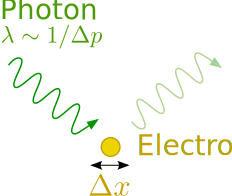
\includegraphics[width=0.75\linewidth]{heisenberg-microscope/simpler-heisenberg-microscope.pdf}
	\end{center}
	\caption[
	  Heisenberg microscope figure motivating sketch, \exclusive
	]{
		A simplified cartoon for the Heisenberg's microscope. The classical 
		argument is, 
		that the uncertainty $\delta x$ of determining the position of the electron
		is related to the wavelength $\lambda \sim h/\Delta p \sin(\varphi)$ of a
		scattering photon within a focussed beam on the electron of an angle 
		$\varphi$.
		Due to a classical optics argument, $\Delta x \sim 
		\lambda/\sin(\varphi)$.
		This motivates the original Heisenberg's uncertainty principle 
		$\Delta x \Delta p \sim h$. In the main text, an electron displacement
		due to gravitational interaction is added.
     }
	\label{fig:heisenberg-microscope}
\end{marginfigure}
%
%
According to the KMM model \cite{KMM95}, the GUP manifests itself via a deformation
of the integration measure in momentum space. Following \eqref{eq:commrel}, the
Hilbert space representation of the identity becomes
\begin{equation}
\mathbb{I}=  \int \frac{\diff^{d-1} \vec{p}}{1+\beta {\vec p}^2}\ \left|p \right>\left< p\right|
\,,
\label{GUPmeasure}
\end{equation}
where $\vec{p}$ is a ($d-1$)-dimensional spatial vector. While momentum operators
preserve their feature as in quantum mechanics, position operators no longer
admit physical eigenstates, as one should expect in the presence of a minimal
resolution length $\sqrt{\beta}$. A closer inspection of (\ref{GUPmeasure})
shows that the measure is suppressed in the ultraviolet regime
\begin{equation}
\mathrm{d}{\cal V}_p \equiv \frac{\mathrm{d}^{d-1} p}{1 + \beta {\vec p}^2} \underset{\beta {\vec p}^2\gg 1}{\overset{}{\approx}}
|{\vec p}|^{\,d-4}\ \mathrm{d}|{\vec p}|.
\label{eq:intvol}
\end{equation}
We note that for $d=4$ one recovers \eqref{eq:kempf}, and the momentum term on
the right-hand side disappears. Conversely for $d>4$, the measure diverges
in the ultraviolet regime. As $d$ increases, the effect of the GUP becomes
increasingly weaker, when being used to improve the
higher dimensional Newtonian potential.

There are, however, other proposals. Gravitational effects in quantum mechanics,
such as the GUP, can be motivated with the Gedankenexperiment of Heisenberg's
microscope \cite{Adl10,Car14}.% (Figure \ref{fig:heisenberg-microscope}).
Specifically, next to the spatial
uncertainty $\Delta x \sim \Delta x_C$
arising from the Compton wavelength of a particle
$\Delta x_\mathrm{C} \sim \lambda \sim 1/\Delta p$,
one can introduce an additional displacement $\Delta x_\mathrm{g}$ for the
electron due to the gravitational interaction with the incoming photon.
By assuming a Newtonian description, ones finds that 
\begin{equation}
\Delta x_\mathrm{g}\sim G_\mathrm{N}\frac{M_{\rm eff}}{r^{2}} \left(\frac{r^2}{c^2}\right) 
\sim G_\mathrm{N}  \Delta p
\sim (\sqrt{\beta})^{2} \Delta p
\end{equation}
for $d=4$, where $M_{\rm eff}=h/(\lambda c)$ is the effective photon mass and
$\sqrt{\beta}\sim \ellp$. The total uncertainty is obtained by adding
$\Delta x_\mathrm{g}$ to the standard quantum uncertainty, namely
$\Delta x=\Delta x_\mathrm{C}+\Delta x_\mathrm{g}$ with 
$\Delta x_\mathrm{C}\sim 1/\Delta p$. Following the reasoning of Scardigli
and Casadio \cite{ScC03}, as well as Carr and Lake
\cite{Car13,Car14,LaC15,LaC16,Carr:2017grh,LaC18}, the extension of the 
above calculation to the case $d>4$ leads to
\begin{equation}
\Delta x_\mathrm{g}
\sim G_\ast \frac{M_{\rm eff}}{r^{d-2}} \left(\frac{r^2}{c^2}\right)
\sim G_\ast \frac{\Delta p}{r^{d-4}}\leadsto \Delta x_\mathrm{g}^{d-3}
\sim L_\ast^{d-2} \Delta p \,,
\label{eq:CLCSgup}
\end{equation}
having assumed $r\sim\Delta x_\mathrm{g}<R_\mathrm{c}$.
The uncertainty relation then reads
\begin{equation}\label{eq:modifGUP}
\Delta x \Delta p \geq \frac{\hbar}{2} \left( 1 + \left( \sqrt{\beta}\, \Delta p \right)^{\frac{d-2}{d-3}} \right),
\end{equation}
where $\sqrt{\beta}\sim L_\ast$. On  the other hand, for
$r\sim\Delta x_\mathrm{g}>R_\mathrm{c}$, the uncertainty relation is
assumed to be that for $d=4$ displayed in \eqref{eq:gup}. From
\eqref{eq:modifGUP} one can show that the momentum space measure
can be expressed as
\begin{equation}
\mathrm{d}{\cal V}_p \equiv \frac{\mathrm{d}^{d-1} p}{1 + (\beta {\vec p}^2)^{\frac{1}{2}\frac{d-2}{d-3}}} \underset{\beta {\vec p}^2\gg 1}{\overset{}{\approx}}
|{\vec p}|^{d-3}\ \mathrm{d}|{\vec p}|,
\label{eq:intvol2}
\end{equation}
for $d>4$. 
This means that in such a scenario the GUP corrections are even
milder than those of the KMM model. However, it assumes a
modified higher dimensional GUP as
\begin{equation}\label{eq:KerrGUP}
\Delta x \Delta p \geq \frac{\hbar}{2} \left( 1 + \left( \sqrt{\beta}\, \Delta 
p \right)^{\frac{d-2}{d-3}} \right) \,.
\end{equation}
Eq. \eqref{eq:KerrGUP} is consistent with what proposed
in \cite{ScC03,Maz13,Car13,Car14,LaC15,LaC16} and clearly reproduces the higher 
dimensional Schwarzschild radii for energies above the terascale.

\begin{marginfigure}
	\includegraphics[width=\linewidth]{figures-from-gup-proceeding/completeness-real-gup-bigger.pdf}
	\caption[
	Completness plot solved with GUP, \publishedIn{Koppel:2017rsf}
	]{Completeness plot with the $(3+1)$-dimensional GUP solution.
	  Compare with Figure~\protect\ref{fig:completeness-intro}.
	  Published in \cite{Koppel:2017rsf}.
	}
	\label{fig:gup-completeness}
\end{marginfigure}

Given the ambiguity in results described above, we proposed another
revision to the Heisenberg microscope in \cite{Koppel:2017rsf}.
From \eqref{eq:CLCSgup} one
obtains that $\Delta x_\mathrm{g}\geq L_\ast$ only for
$\Delta p \geq M_\ast$. As a result, for any $\Delta p \leq M_\ast$
the gravitational uncertainty is negligible,
$\Delta x_\mathrm{g}<\Delta x_\mathrm{C}< R_\mathrm{c}$. In such a
regime the typical interaction distance is controlled by the
Compton wavelength, $r\sim \Delta x_\mathrm{C}\sim 1/\Delta p$.
In Figure \ref{fig:gup-completeness}, this complies with
``approaching'' the quantum gravity scale from the left
(Sub-Planckian Regime).
This implies that
\begin{equation}
\Delta x_\mathrm{g}
\sim G_\ast \frac{M_{\rm eff}}{r^{d-2}} \left(\frac{r^2}{c^2}\right)
\sim G_\ast \frac{\Delta p}{r^{d-4}}
\sim L_\ast^{d-2} \Delta p^{d-3}.
\end{equation}
The above relation relaxes the proportionality condition between
$\Delta x_\mathrm{C}$, $\Delta x_\mathrm{g}$ and the radius of the
Tangerlini-Schwarzschild black hole \cite{Koppel:2017rsf}. As a
byproduct, however, one obtains a stronger correction in momentum
space since gravity will begin to probe extra dimensions at scales
$r< R$. This can be inferred from the condition
\begin{equation}
\mathrm{d}{\cal V}_p \equiv \frac{\mathrm{d}^{d-1} p}{1 + (\beta {\vec p}^2)^{\frac{d-2}{2}}} \underset{\beta {\vec p}^2\gg 1}{\overset{}{\approx}}
\ \mathrm{d}|{\vec p}|,
\label{eq:intvol3}
\end{equation}
namely it is uniformly suppressed irrespective of the number
of dimension~$d$. 

\begin{table}[b]
	\begin{tabularx}{\linewidth}{llll}
		\firsthline
		Eq. & Short name  & Volume element & Large $p$ limit \\
		\hline 
		& No GUP   & $\d^{d-1} p$           & $p^{d-2} \d p$ \\
		\eqref{eq:intvol2} & Carr     & $\d^{d-1} p / (1 + (\sqrt \beta~p)^{(d-2)/(d-3)})$ & $p^{d-3} \d p$ \\
		\eqref{eq:kempf} & KMM      & $\d^{d-1} p / (1 + (\sqrt \beta~p)^2)   )$ & $p^{d-4} \d p$  \\
		\eqref{eq:intvol3} & Adjusted & $\d^{d-1} p / (1 + (\sqrt \beta~p)^{d-2})$ & $\d p$ \\
		\hline
	\end{tabularx}
	\caption[
	  Overview of different GUP formulations in higher dimensions
	]{
	  An overview of different GUP formulations in higher dimensions
	  (also ``no GUP'' is considered, for reference), with their 
	  mathematical definition (including a text reference) and their
	  classical limit.
	}
\end{table}

There are three arguments in support of the above reasoning. First,
the requirement that a  quantum gravity correction
$\Delta x_\mathrm{g}$ is proportional to a classical quantity like
the Tangerlini-Schwarzschild black hole is not fully consistent.
It makes sense only for $r > R$, namely at length scales at which
gravity becomes classical and only four dimensions are visible. 
Second, investigations of string scattering showed that the
position-momentum uncertainty relation is of the form \eqref{eq:gup}
\cite{ACV89,ACV93}. Such a result has, however, been obtained
in the eikonal limit and higher order corrections for the ultraviolet
regime of momentum space are expected. Third, the above corrections
are consistent with the algebra proposed in \cite{Maz12,DMS15,Maz15}.

In the remainder of this paper, we present higher dimensional black
hole solutions that emerge from the non-local field equations
\eqref{eq:nleinstein} that account for GUP effects following from
\eqref{eq:intvol}, \eqref{eq:intvol2} and \eqref{eq:intvol3}
according to the method first proposed in \cite{IMN13}.


\section{Revised GUP in higher dimensions}\label{sec:revised-gup}
In this section, the imprint of the improved higher dimensional GUP
\eqref{eq:intvol3} is studied.
%
As a start, one has to determine the corresponding operator $\mathbb{G}\left(L^2\Box\right)$, namely
\begin{equation}
\mathbb{G}\left(L^2\Box\right)=\frac{G_\ast}{1-\left(L^2\Box\right)^{\frac{n-1}{2}}}\equiv G_\ast \sum_{N=0}^\infty \left[\left(L^2\Box\right)^{\frac{n-1}{2}}\right]^N,
\end{equation}
where, in case of half integer exponents, $\frac{n-1}{2}=\frac{3}{2}, \frac{5}{2}, \frac{7}{2}, \dots$, the following Schwinger representation can be used to express  powers of an arbitrary operator, $\hat{O}$:
\begin{equation}
\hat{O}^{\alpha}=\frac{1}{\Gamma(-\alpha)}\int_0^\infty ds \ s^{-\alpha - 1} \ e^{-s\hat{O}}, \quad \alpha\in \mathbb{R}\setminus\mathbb{N}.
\end{equation}
The resulting energy momentum tensor has the same form of that presented in
Section~\ref{sec:lxd-kmm}, namely
$\mathbb{T}_\mu^\nu=\mathrm{diag} \left(-\rho, p_r, p_\perp, p_\perp, \dots\right)$
with $p_r=-\rho$ and $p_\perp=-\rho-\frac{r}{n-1} \left(\frac{\diff \rho}{\diff r}\right)$.
The energy density and the other components have, however, a different profile.
To determine $\mathbb{T}_0^0$, one has to consider the integral
\begin{align}
\mathbb{T}^0_0(\vec{x}) = -\rho(\vec{x})=-
\frac{M}{(2\pi)^{n}} \int \frac{\diff^n\vec{p}}{1 + 
	(\sqrt{\beta} p)^{n-1} }e^{i \vec{x}\cdot\vec{p}}
\label{eq:t00newgup}
\end{align}

\subsection{Calculation of the energy density}
The modified source term can be written as a Fourier Transform of a spherically 
symmetric function 
$\mathcal{F}\left\{ f(p) \right\}(x) \equiv \frac{1}{(2\pi)^{n/2}} \int\diff^n 
\vec{p}\ f(p) e^{i \vec{x}\cdot\vec{p}}$
\begin{align}
\rho(x) &= \frac{M}{(2\pi)^{n}} \int \frac{\diff^n\vec{p}}{1 + 
(\sqrt{\beta} p)^{n-1} }e^{i \vec{x}\cdot\vec{p}} \\
&= \frac{M}{(2\pi)^{n/2}} \mathcal{F}\left\{ \frac{1}{1+(\sqrt{\beta} p)^{n-1}} 
\right\}(x) \\
&= \frac{M}{(2\pi)^{n/2}} \frac{1}{x^{\frac{n-2}{2}}} \int_0^\infty \diff p\, 
p^{\frac{n}{2}}
    \frac{1}{1+(\sqrt{\beta} p)^{n-1}} J_{\frac{n-2}{2}}(x p)\ ,
    \label{eq:source}
\\
&= \frac{M \beta^{-n/2}}{(2\pi)^{n/2}} \frac{1}{z^{\frac{n-2}{2}}} 
\int_0^\infty 
\diff q\, 
q^{\frac{n}{2}}
\frac{1}{1+q^{n-1}} J_{\frac{n-2}{2}}(zq)\ ,
\label{eq:rho-ndim-integral}
\end{align}
where the Bessel function of first kind $J_\alpha(x)$ comes from 
integrating out the angles. Due to the complexity of th adjusted
GUP, no general closed algebraic expressions could be derived and
instead a numerical approach was taken.

By introducing the dimensionless variables $z=r/\sqrt{\beta}$ and $q=\sqrt{\beta}p$, the above integral reads:
\begin{align}
\rho(z) 
&= \frac{M \beta^{-n/2}}{(2\pi)^{n/2}} \frac{1}{z^{\frac{n-2}{2}}} 
\int_0^\infty 
\diff q\, 
q^{\frac{n}{2}}
\frac{1}{1+q^{n-1}} J_{\frac{n-2}{2}}(zq) \,.
\label{eq:rho-ndim-integral}
\end{align}
For small arguments the Bessel function behaves as
\begin{equation}
J_{\alpha }(z)\approx {\frac {1}{\Gamma (\alpha +1)}}\left({\frac {z}{2}}\right)^{\alpha }.
\end{equation} 
This means the integral is well defined at the lower bound.
For large arguments the Bessel function can be written
\begin{equation}
J_{\alpha }(z)\approx \frac{1}{|z|}.
\end{equation} 
This guarantees the expected convergence of the integral for $q\to\infty$.
On these grounds, the numerical evaluation is possible by integrating from
zero-crossing (i.e. the $z$ where $J_\alpha(z)=0$) to zero-crossing in order
to stabilize the integration and to ensure convergence
(Figure~\ref{fig:BesselIntegrator}). For numerical
purposes, the density can be approximated as
\begin{align}
\rho(z) 
&\approx \frac{M \beta^{-n/2}}{(2\pi)^{n/2}} \frac{1}{z^{\frac{n-2}{2}}} 
\sum_{k=0}^K
\sum_{i=0}^{I\Delta q}
\Delta q~
q_{i,k}^{\frac{n}{2}}
\frac{1}{1+q_{i,k}^{n-1}} J_{\frac{n-2}{2}}(zq_{i,k})
\,.
\label{eq:rho-ndim-integral-discrete}
\end{align}
%
\begin{marginfigure}
	\includegraphics[width=\linewidth]{svens-new-mma-figures/BesselIntegrator.pdf}
	\caption[Besselintegrator, with Mathematica, \exclusive]{
		The key part for a successful numerical integration of the highly oscillatory
		Hankel transformation $\int_0^\infty f(x) J_\alpha(xy)$
		with kernel $f(x)$ and $\lim_{x\to \infty} f(x)=0$
		is to correctly track the zero crossings of the oscillating Bessel function.
		Here, every color indicates a seperate integration domain.
	}\label{fig:BesselIntegrator}
\end{marginfigure}%
%
Here, $K\in \mathbb{N}$ are the number of zero crossings taken into account
(typical values are $K=3000$),
and $I\in \mathbb{N}$ are the total number of integration support points, each given by 
$q_{i,k}=j_k + i\Delta q$, with $j_k$ the coordinate of the $k$th root of
$J_{(n-2)/2}(zq)$.
Clearly, with $I,K\to\infty$ and $\Delta q\to 0$, the continous
integral \eqref{eq:rho-ndim-integral} is recovered. We checked convergence with
different grid sizes $I,K \in \{10^2, 10^3, 10^4\}$. 
For the actual numerical integration, a standard Gaussian quadrature rule is applied.
The function values
$\rho_{\beta,n}(z)$ are then available on a discrete sample set $\{z_i\}\subset 
\mathbb R$ with arbitrary resolution and coverage.
%
With this numerical approach, one can also integrate the mass distribution,
\begin{equation}
    \mathcal{M}(r) = M \int_{B_r}\diff^n \vec{x}\,\rho_\beta(x) = 
    M A_{n-1}\int_0^r\diff x\,x^{n-1}\rho(x)\,,
    \label{eq:modGUPmass}
\end{equation}
where $A_{n-1}=2\pi^{n/2}/\Gamma(n/2)$.
Again, this integral is carried out numerically as a cumulative sum in a
straightforward manner. From the matter distribution, one obtains the metric
coefficients \eqref{eq:tangherlini}.
Figure~\ref{fig:adjustedGUP-starters} shows the mass distribution
$\mathcal{M}(r)$ for a number of extra dimensions. 
Interestingly the case $n=3$ is the only having $\mathcal{M}(r)$ described
by a monotonic increasing function. For $n>3$ there is a surprising new
behavior: the function oscillates with an amplitude that increases with $n$
and decreases with $r$. A naive interpretation of the oscillations is the
presence of negative contributions in the energy density for some regions
close to the spatial origin. 
We recall that such negative density regions are not a remote possibility,
at least during the early stages of the Universe, for the presence of strong
quantum fluctuations of the spacetime manifold \cite{MTY88,Mann97}.

\begin{figure}[t]
	% This new figure of Sven replaces Marcos gup-figures/g00kempf.pdf
	\includegraphics[width=\linewidth]{svens-new-python-figures/adjusted-gup-mass-distributions.pdf}
	\caption[
	Revised GUP, Mass distributions \publishedIn{Knipfer2019}
	]{
      Mass distributions \protect\eqref{eq:modGUPmass} for the revised GUP model
      \protect\eqref{eq:intvol3}, for different number of spatial dimensions $n$.
      While $n=3$ complies with a smeared Heaviside function, there are
      oscillations around the spacetime mask, which however quickly decline
      for larger radii (the scale is $r_0 \sim L_* \sim L_\text{Pl}$).
      Note that for larger radii, even regions with $\mathcal M(r)<0$ are
      possible.
	}
\end{figure}%
\begin{figure}[b]
	\caption[
	Revised GUP, Temperature profiles \publishedIn{Knipfer2019}
	]{
		Temperature profiles (defined as in \protect\eqref{eq:temp-higher-dim-def}, with the
		revised GUP of Section~\protect\ref{sec:revised-gup}) in different number
		of dimensions, compared with the respective Schwarzschild-Tangherlini
		temperature (dashed lines). The red disks mark local maxima, while the blue
		disk marks the evaporation endpoint. Since the abscissa is given in multiples
		of the respective endpoint radius, all temperatures end at the same point.
	}\label{fig:adjustedGUP-starters}
	\includegraphics[width=\linewidth]{svens-new-python-figures/adjusted-gup-temperatures.pdf}
\end{figure}

One can also advance another interpretation based on the presence of $n-1$
tachyon states of mass, $i/\sqrt{\beta}\sim i M_\ast$, emerging from the
poles of the integrand function in \eqref{eq:t00newgup}. As a consequence
the energy density $\rho(\vec{x})$, despite being positive defined at
the origin,  oscillates around zero for larger values of $r$. 
A possible explanation  can be found in the fact that the GUP captures
only part of the non-perturbative corrections of quantum gravity. 
Interestingly, such oscillations of the Newtonian potential have been
found in a variety of formulations aiming to amend Einstein gravity.
These include $f(R)$-gravity \cite{NoO2003,Olmo2005,Faraoni96,CST2007,NoO2007,CENOSZ2008,CDLF2010,BeG2011,Schell2016},
string induced, ghost free, non-local gravity \cite{EKMaz2016,FroZ2016}
and other non-local formulations \cite{KeMa2014}.   
On the other hand, in the low energy limit for which only the $3$ spatial
dimensions are visible, the oscillations disappear as expected in similar
quantum gravity contexts \cite{HaH02,Perivo16}.
%since there are not enough tachyon states to produce long distance oscillations . 
This scenario is consistent with the  fact that GUP corrections descend
from the  eikonal limit of string collisions at the Planck
scale \cite{ACV89,ACV93,ACV87,ACV88,ACV90,GrM88,GrM87}.

Even if the above effects are just a short-scale, quantum mechanical
property of the solution, they have important repercussions on the
thermodynamics of the system. The profile of the  temperature  is
presented in Fig.~\ref{fig:adjustedGUP-starters}. One can see that the
oscillations of $\mathcal{M}(r)$  produce temperature oscillations
corresponding to phase transitions from negative to positive heat
capacity phases. The resulting variable luminosity of the black hole
can be termed as a \textit{light-house effect}. Interestingly such an
effect increases with $n$. For lower $n$  one obtains small amplitude
oscillations of the temperature. 

\subsection*{Different endpoints for small and big black holes}
More importantly, further scenarios are possible. In Figure \ref{fig:adjusted-gup-n8-indepth},
the case of $d=9$ space time dimensions is depicted. For this number of dimensions, two scenarios are
possible, depending on the black hole mass. For big mass black holes, $M>M_1$, the temperature oscillation determined an anticipated shut-down of the Hawking emission with the formation of zero temperature remnants; we refer to the masses of these zero temperature configurations as $M_1 = 3.73 \times 10^6 M_*$.
Such a large mass regime is a characterized by a rich horizon structure. For $M>2.14 M_1$, there are just two horizons, an event horizon, $r_+$ and an inner Cauchy horizon, $r_-$. For $M=2.14 M_1$, the function $g_{00}$ admits a double zero between the aforementioned two horizons. For smaller masses  $M_0<M<2.14 M_1$, the function $g_{00}$ admits $4$ simple zeros, \textit{i.e.}, $r_-<r_2<r_3<r_+$. Finally for $M=M_1=3.73 \times 10^6 M_*$, there is the merge between $r_3$ and $r_+$ that form a double zero, corresponding to the extremal configuration, \textit{i.e.}, the end stage of the evaporation.
In terms of horizon radii, there is a regime that do not occur, i.e. $r_i < r < r_1$, where $r_1 =5.93r_0$ is the
size of the large black hole evaporation endpoint, and an intermediate radius $r_i=5.0r_0$.
For even smaller masses, $M<M_1$ however, there are horizons again, $r_\pm$, that eventually merge in a new extremal configuration $r_0=r_-=r_+$ for $M=M_0=5.15 \times 10^3 M_*$.

\begin{margintable}
	\centering
	\begin{tabular}{clll}
		\toprule
		{$n$} & $\sqrt{\beta_0}$ & $r_0$ & $m_0$ \\
		\midrule
		{3}        & 1.45         & 2.60      & 2.42\\
		{4}        & 0.71         & 1.18      & 5.31\\
		{5}        & 0.48         & 0.85      & 7.43\\
		{6}        & 0.38         & 0.71      & 8.88\\
		{7}        & 0.32         & 0.64      & 9.89\\
		{8}        & 0.27         & 0.59      & 10.6\\
		{9}        & 0.25         & 0.56      & 11.1\\
		{10}       & 0.23         & 0.55      & 11.5 \\
		\bottomrule
	\end{tabular}
	\caption[Self-completeness values for the adjusted GUP]{
		Numerical values for $\sqrt{\beta_0}$ in the self complete
		paradigm. These values are of no further meaning,
		they just demonstrate that it is possible to apply the
		self-complete paradigm in any number of extra dimensions.
	}\label{table:self-completeness-adjusted-gup}
\end{margintable}

Here, the self-completeness paradigm was implemented by choosing the free
parameter $\beta$ in a way, that the Compton wavelength
$\lambda_\text{C} = h/M_0c$ of the zero temperature configuration is equal
to its horizon radius $r_0$. The determination of $\beta$ cannot even be 
done analytically in 3+1 dimensions. Therefore, numerical results are
given in Table \ref{table:self-completeness-adjusted-gup}.
%From this equation we get $\beta$ for different dimensions:

\begin{figure*}[t]
	% This new figure of Sven replaces Marcos gup-figures/g00kempf.pdf
	\makebox[\textwidth][c]{ % overwidth figure
		\includegraphics[width=1.1\linewidth]{svens-new-python-figures/alternative-adjusted-gup-n8-indepth.pdf}
	}% end of overwidth makebox
	\caption[
	  GUP potential for $n=8$, selfmade (Python), \exclusive
	]{
		Comprehensive presentation of the possible configurations of the
		revised GUP model (Section~\protect\ref{sec:revised-gup}) in $n=8$ spatial
		dimensions. The central panel shows the temperature (solid line) compared to
		the Schwarzschild-Tangherlini solution (dashed). There are two regimes,
		shaded in red (small black holes) and green (big black holes).
		Typical gravitational potentials for different masses for the small black
		holes are depicted in the left panel, while the right panel holds the
		same for the large black holes. Dots always denote horizons.
		The different scenarios are discussed in the main text.
		
		Appendix \protect\ref{apx:adjusted-gup} shows this diagram in another representation
		and also covers the $n=9$ case, for comparison.
	}\label{fig:adjusted-gup-n8-indepth}
\end{figure*}


In conclusion, there is a small mass and a large mass regime for black holes. The former can be thought to form due the high density fluctuation of the early Universe \cite{CaH74} or by de Sitter space decay, as predicted in terms of the instanton formalism \cite{MaR95,BoH96,MaN11}.

We have also to note that the presence of two remnant masses posits an ambiguity of the scale at which gravity may be self complete \cite{MuN12,DFG11,DFG12,SpA11,Nic2018}. In other words gravity is able to mask singularities by covering them with an extremal configuration but the latter has no unique mass scale.


\section{Summary} % Summary were Conclusions
The fact that the black hole temperature diverges for small black holes is one 
of the indicators that
a theory of quantum gravity is needed. The Generalized Uncertainty Principle is
a quantum gravity effect and modifies this behavior (SCRAM phase).
Since the GUP can for example be motivated by string theory which needs extra 
dimensions this strongly suggests
that the cure of the temperature divergence should also work in higher 
dimensions.

In 3+1 dimensions the GUP gives rise to a SCRAM phase for Planckian black holes.
We showed that the  GUP as it has been used in the 3+1 dimensional case does 
not give rise to SCRAM phase in higher dimensions. However, we note that in
the 4+1 dimensional case, the GUP gives rise to a conical singularity.
We generalized the GUP to higher dimensions in the form 
$1/(1+(\sqrt{\beta}p)^{n-1})$, with $n$ spatial dimensions,
motivated by the reasoning in an earlier work~\cite{Koppel:2017rsf}
In this revised GUP we recovered the SCRAM phase.

We also found that there are new oscillations in the density $\rho(r)$ around 
zero. These oscillations lead to oscillations in the mass function $M(r)$, but are
dampened in the metric $g_{00}(r)$.
Nevertheless they again show up in the temperature which now shows a Lighthouse 
Effect of oscillating temperature around the Planck size. Starting at
8+1 dimensions, there are additional zeroes of the temperature, giving rise to
a complex phase structure, where the small black holes can be formed in the
primordial universe.

